\documentclass{article}
\usepackage{v-test-paper}
%\renewcommand{\ans}{\quad}
%\def\ansint#1{\quad}
\title{Module-Test(Physics)\\[-15mm]}
\date{}
\usepackage{multicol}
%	TOPICS
% -> Work Done
% -> Potential Energy
% -> Kinetic Energy
% -> Power : Average : Instantaneous

\begin{document}

\maketitle

\jeeSectionA

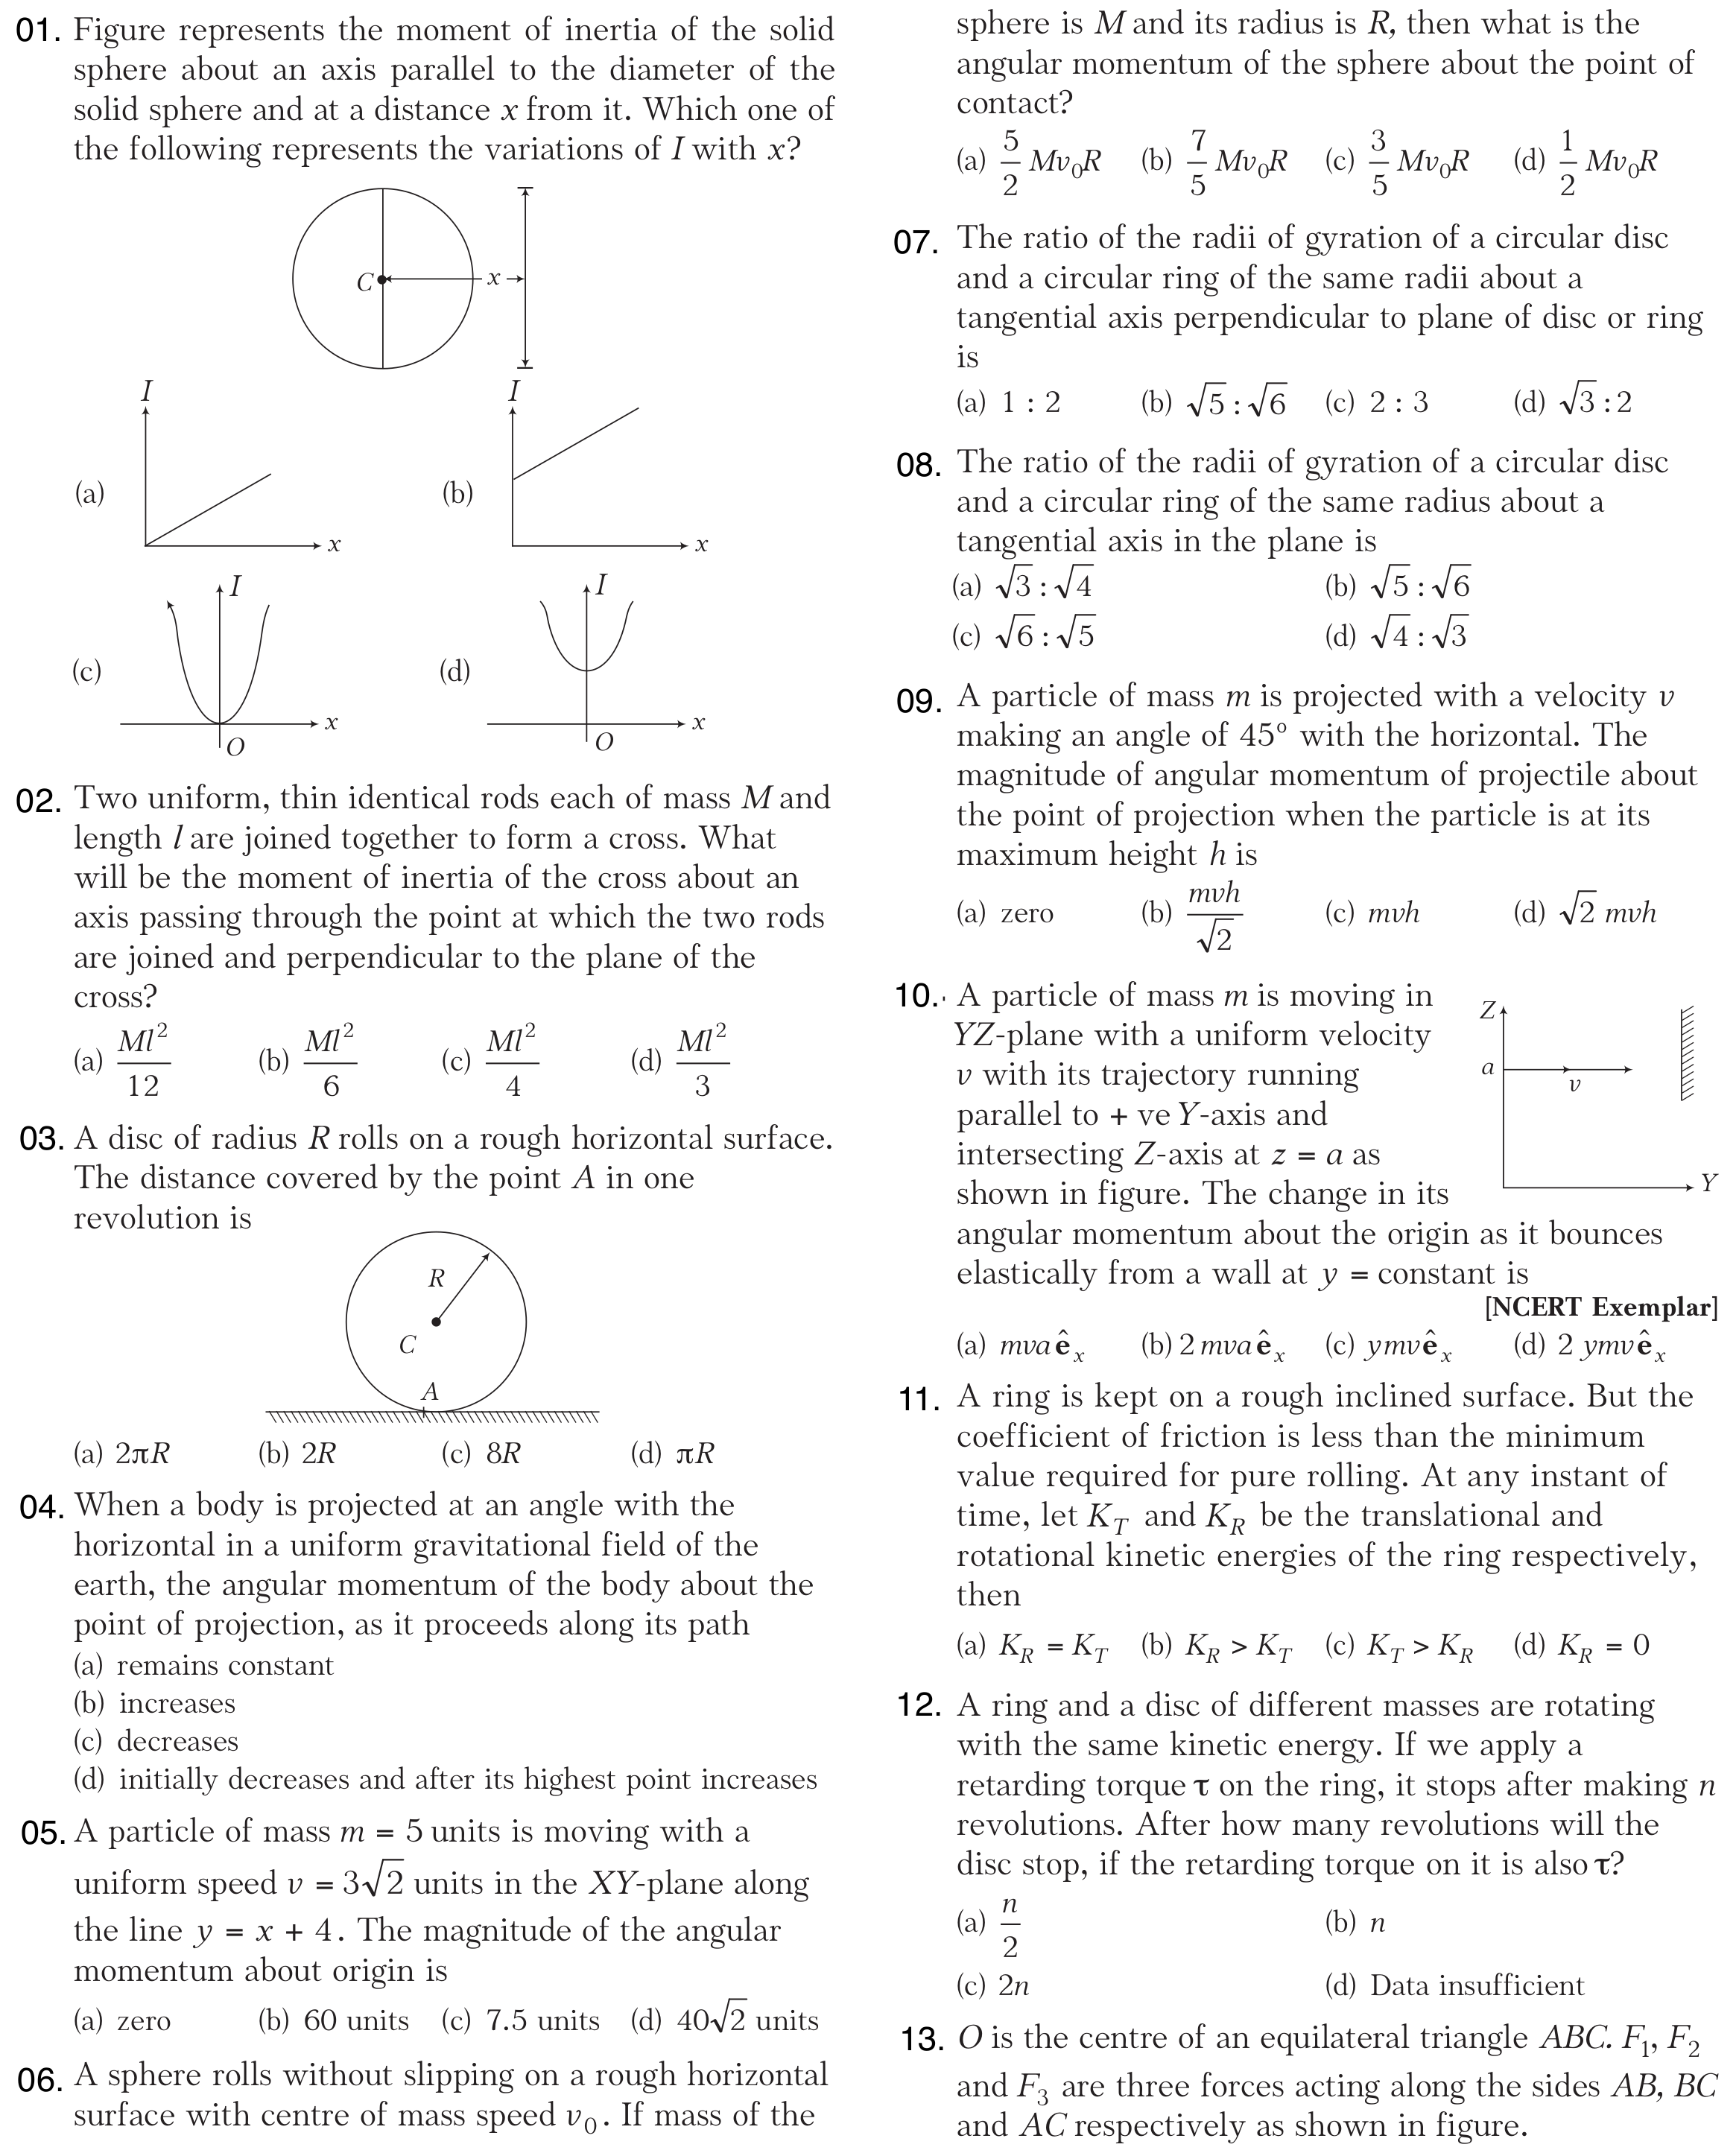
\includegraphics[trim={0.25cm 0 0 0},clip, width=170 mm]{1-13.png}
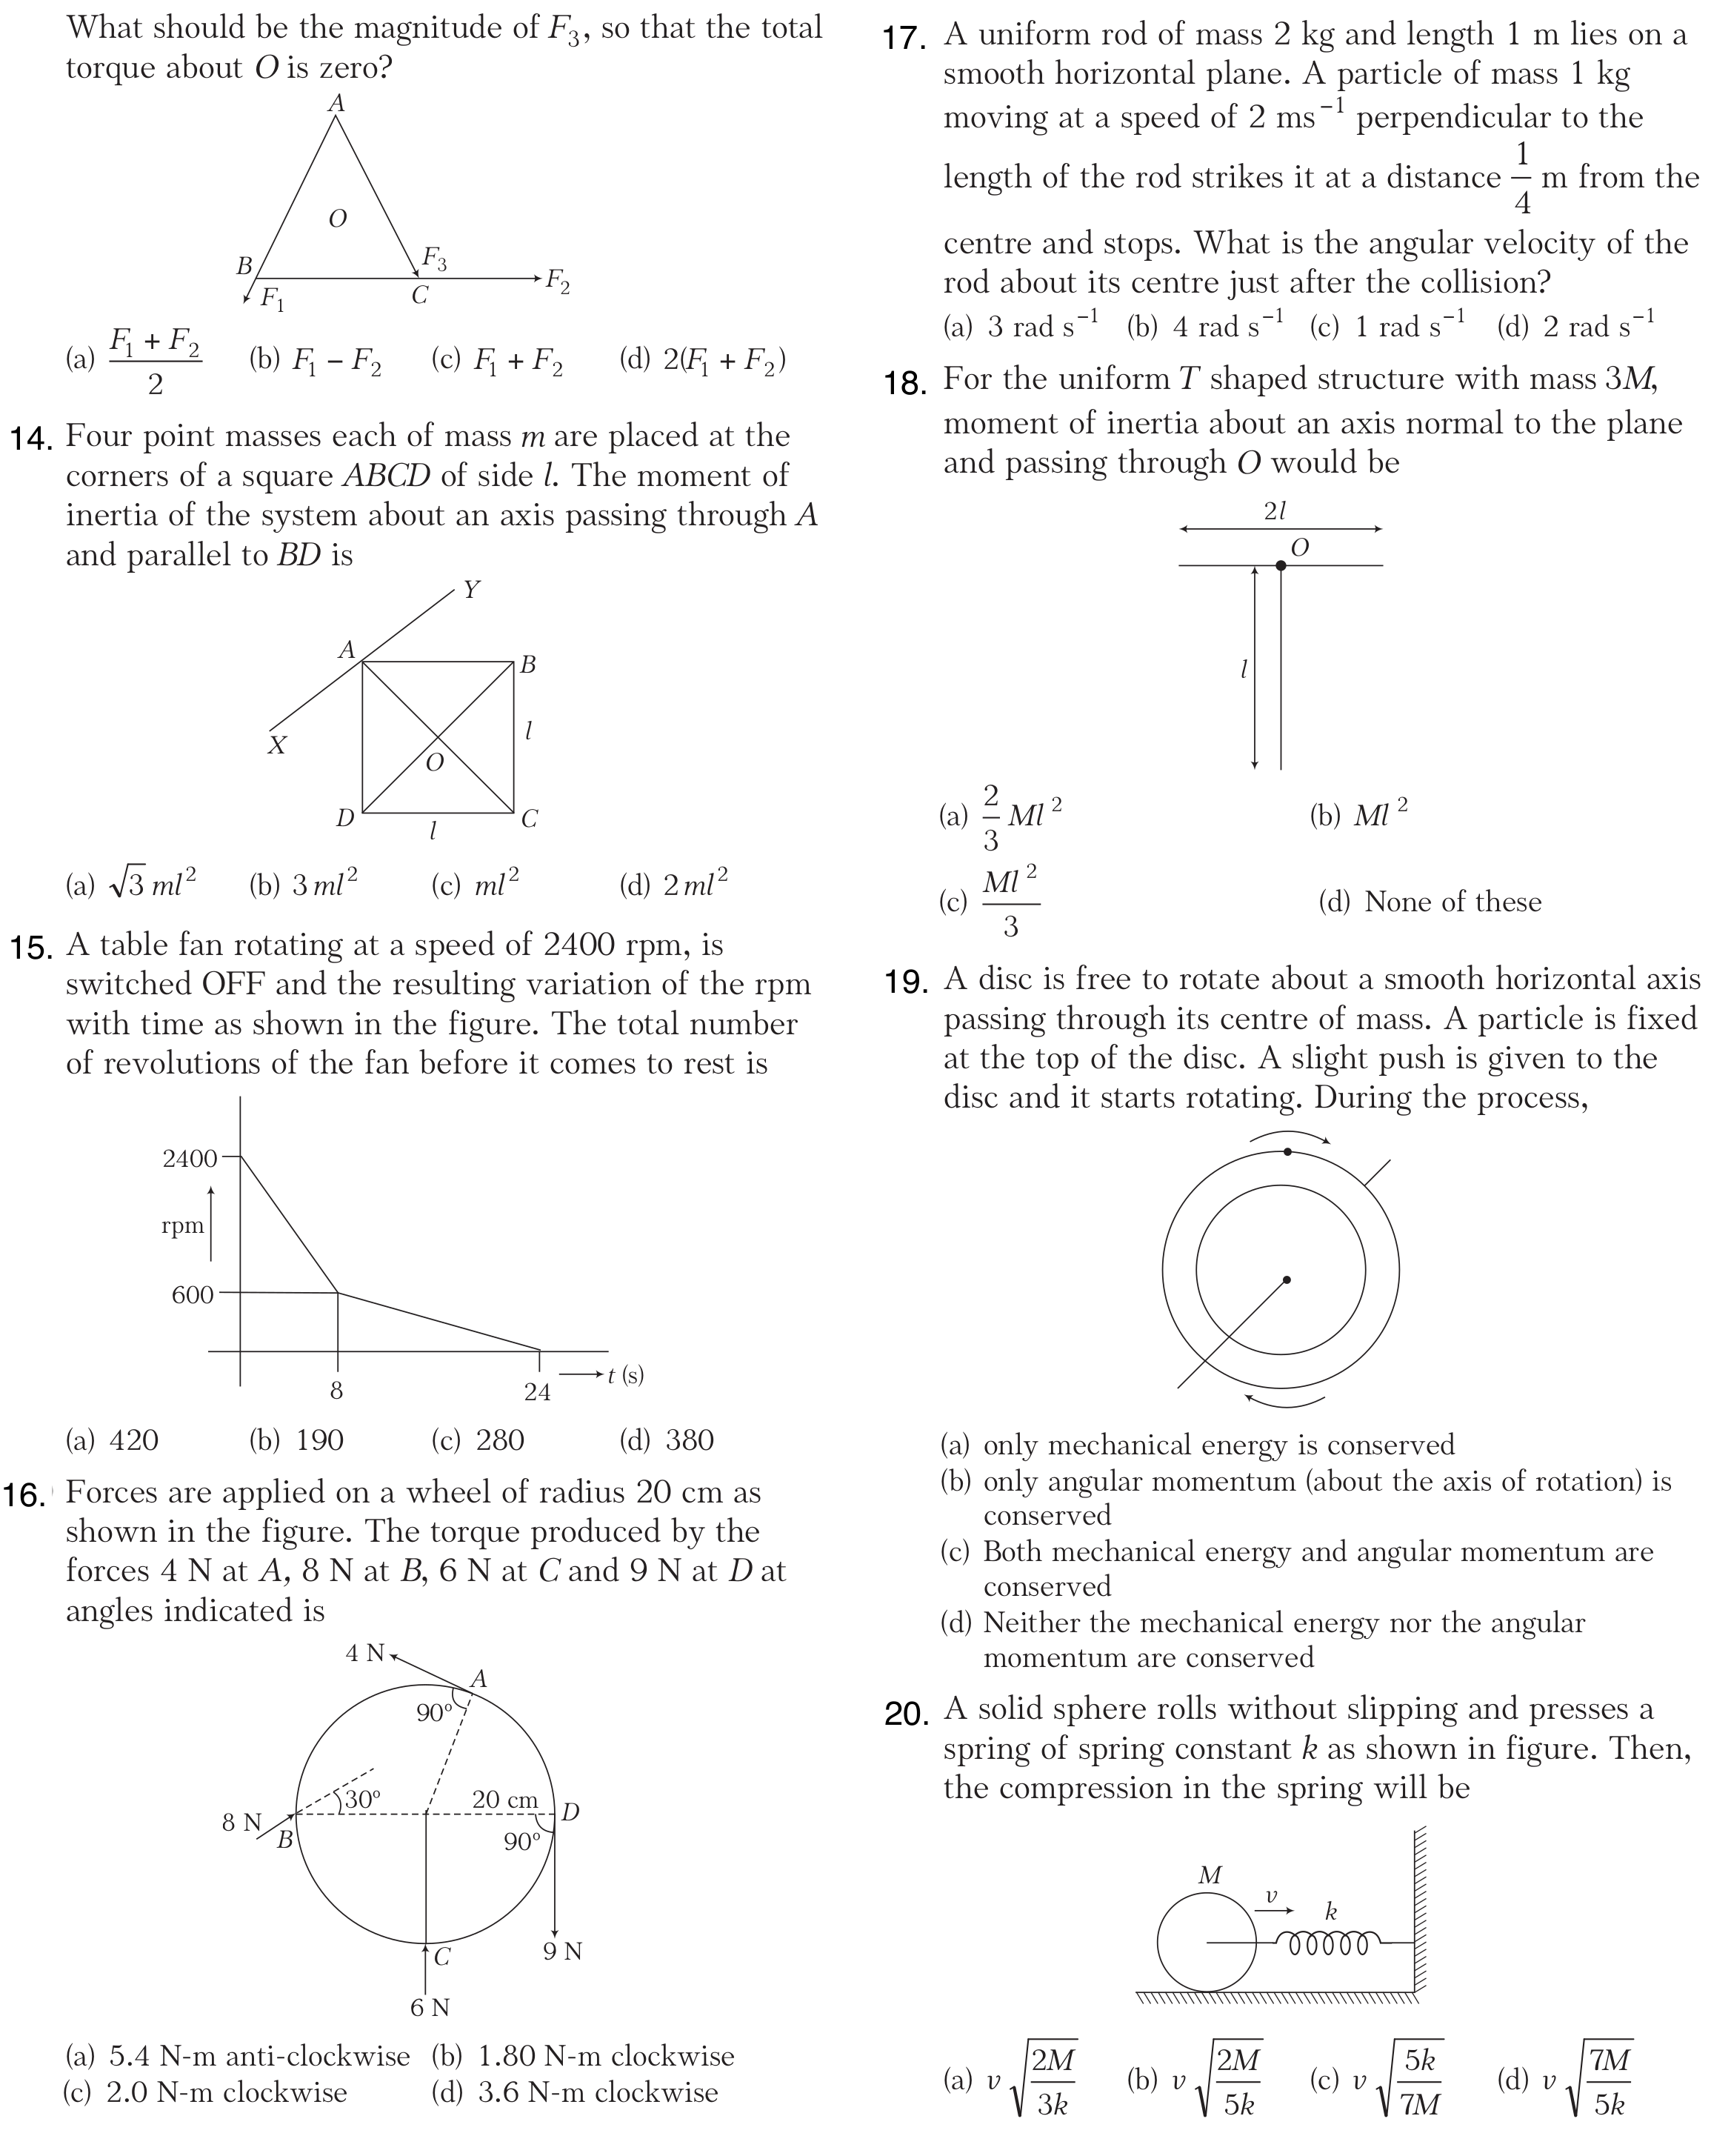
\includegraphics[trim={0.25cm 0 0 0},clip, width=170 mm]{14-20.png}
\jeeSectionB
\begin{enumerate}\addtocounter{enumi}{20}
\item If the rotational kinetic energy of a body is increased by $300\%$, then determine percentage increase in its angular momentum.

\item If the radius of the earth contracts to half of its present value without change in its mass, what will be the new duration of the day?

\item A disc of radius $2 \m$ and mass $100 \kg$ rolls on a
horizontal floor. Its centre of mass has speed of
$0.2 \mps$. How much work is needed to stop it?

\item A uniform circular disc of radius $50 \cm$ at rest is free to turn about an axis which is perpendicular to its plane and passes through its centre. It is subjected to a torque which produces a constant angular acceleration of $2 \text{rad}/\s^{-2}$ . Its net acceleration (in $\mpss$) at the end of $2 \s$ is approximately

\item An explosion breaks a rock into three parts in a horizontal plane. Two of them go off at right angles to each other. The first part of mass $1 \kg$ moves with a speed of $12 \mps$ and the second part of mass 2 kg
moves with speed of $8 \mps$. If the third part flies off with speed of $4 \mps$ , then its mass is

\item A body of mass $4 \kg$ moving with velocity $12 \mps$ collides with another body of mass $6 \kg$ at rest. If two bodies stick together after collision, then the loss of kinetic energy of system is $k$ then $10k$ is

\item Body A of mass $4\m$ moving with speed u collides
with another body B of mass $2\m$ at rest. The collision
is head on and elastic in nature. After the collision,
the fraction of energy lost by the colliding body A is $k$, then $9k$ is

\item Two particles of masses $5 \kg$ and $10 \kg$ respectively are attached to the two ends of a rigid rod of length $1 \m$ with negligible mass. The centre of mass of the system from the $5 \kg$ particle is nearly at a distance in $\cm$ is

\item A moving block having mass $m$, collides with another stationary block having mass $4m$. The lighter block comes to rest after collision. When the initial velocity of the lighter block is $v$, then the value of coefficient of restitution ($e$) multiplied by $100$ will be


\item Body of mass $M$ is much heavier than the other body
of mass $m$. The heavier body with speed $v$ collides
with the lighter body which was at rest initially
elastically. The speed of lighter body after collision is $kv$ then $k$ is
\end{enumerate}

\pagebreak



\begin{center}
\texttt{Module-Test-12\\Physics(Answer)}
\begin{multicols}{2}
\begin{enumerate}
	\item (d)
	\item (b)
	\item (c)
	\item (b)
	\item (b)
	\item (b)
	\item (d)
	\item (b)
	\item (b)
	\item (b)
	\item (c)
	\item (b)
	\item (c)
	\item (b)
	\item (c)
	\item (b)
	\item (a)
	\item (b)
	\item (a)
	\item (d)
	\item $100$
	\item $6$
	\item $3$
	\item $8$
	\item $5$
	\item $1728$
	\item $1$
	\item $67$
	\item $25$
	\item $2$
\end{enumerate}
\end{multicols}
\end{center}



\end{document}
